% !TeX spellcheck = de_DE
\documentclass{uebung_cs}
\usepackage{algo121}
\blattname{\emoji{star}-Aufgabe: Sekundärstruktur}

%%%%%%%%%%%%%%%%%%%%%%%%%%%%%%%%%%%%%%%%%%%%%%%%%%%%%%%%%%%%%%%%%%%%%%%%%%%%
\begin{document}

\textit{\footnotesize For an English version of this exercise, see [\href{https://jeffe.cs.illinois.edu/teaching/algorithms/book/Algorithms-JeffE.pdf}{Erickson}, page 149]}.

\emph{Ribonucleic acid} (RNA) ist eine lange Kette von Millionen Nukleotiden oder \emph{Basen} von vier verschiedenen Typen:
Adenin (\verb|A|), Cytosin (\verb|C|), Guanin (\verb|G|), und Uracil (\verb|U|). Die \emph{Sequenz} eines RNA-Moleküls ist eine Zeichenkette $b[1\dots n]$, wobei jedes Zeichen $b[i]\in\{\texttt{A}, \texttt{C}, \texttt{G}, \texttt{U}\}$ zu einer Basis korrespondiert.
Zusätzlich zu den chemischen Verbindungen zwischen adjazenten Basen in der Sequenz können auch Wasserstoffbrückenbindungen zwischen manchen Basenpaaren entstehen.
Die Menge der gebundenen Basenpaare heißt die \emph{Sekundärstruktur} des RNA-Moleküls.

Wir sagen, dass zwei Basenpaare $(i,j)$ und $(i',j')$ mit $i<j$ und $i'<j'$ sich \textbf{\emph{überlappen}}, wenn $i<i'<j<j'$ oder $i'<i<j'<j$ gilt. In der Praxis überlappen sich die meisten Basenpaare nicht. Überlappende Basenpaaren bilden sogenannte Pseudoknoten in der Sekundärstruktur, die essenziell für bestimmte Funktionen der RNA sind, aber schwierig vorhergesagt werden können.

Wir wollen jetzt die bestmögliche Sekundärstruktur für eine gegebene RNA-Sequenz berechnen. Wir nehmen das folgende vereinfachte Modell der Sekundärstruktur an:
\begin{itemize}
    \item Jede Basis kann mit höchstens einer weiteren Basis eine Bindung eingehen.
    \item Nur \verb|A-U| Paare und \verb|C-G| Paare können gebunden sein.
    \item Paare der Form $(i,i+1)$ und $(i,i+2)$ können sich nicht binden.
    \item Gebundene Basenpaare können sich nicht überlappen.
\end{itemize}
Diese letzte (und am wenigsten realistische) Einschränkung erlaubt es uns, die Sekundärstruktur der RNA als eine Art fetten Baum zu visualisieren:
\begin{figure}[hp]
    \begin{center}
        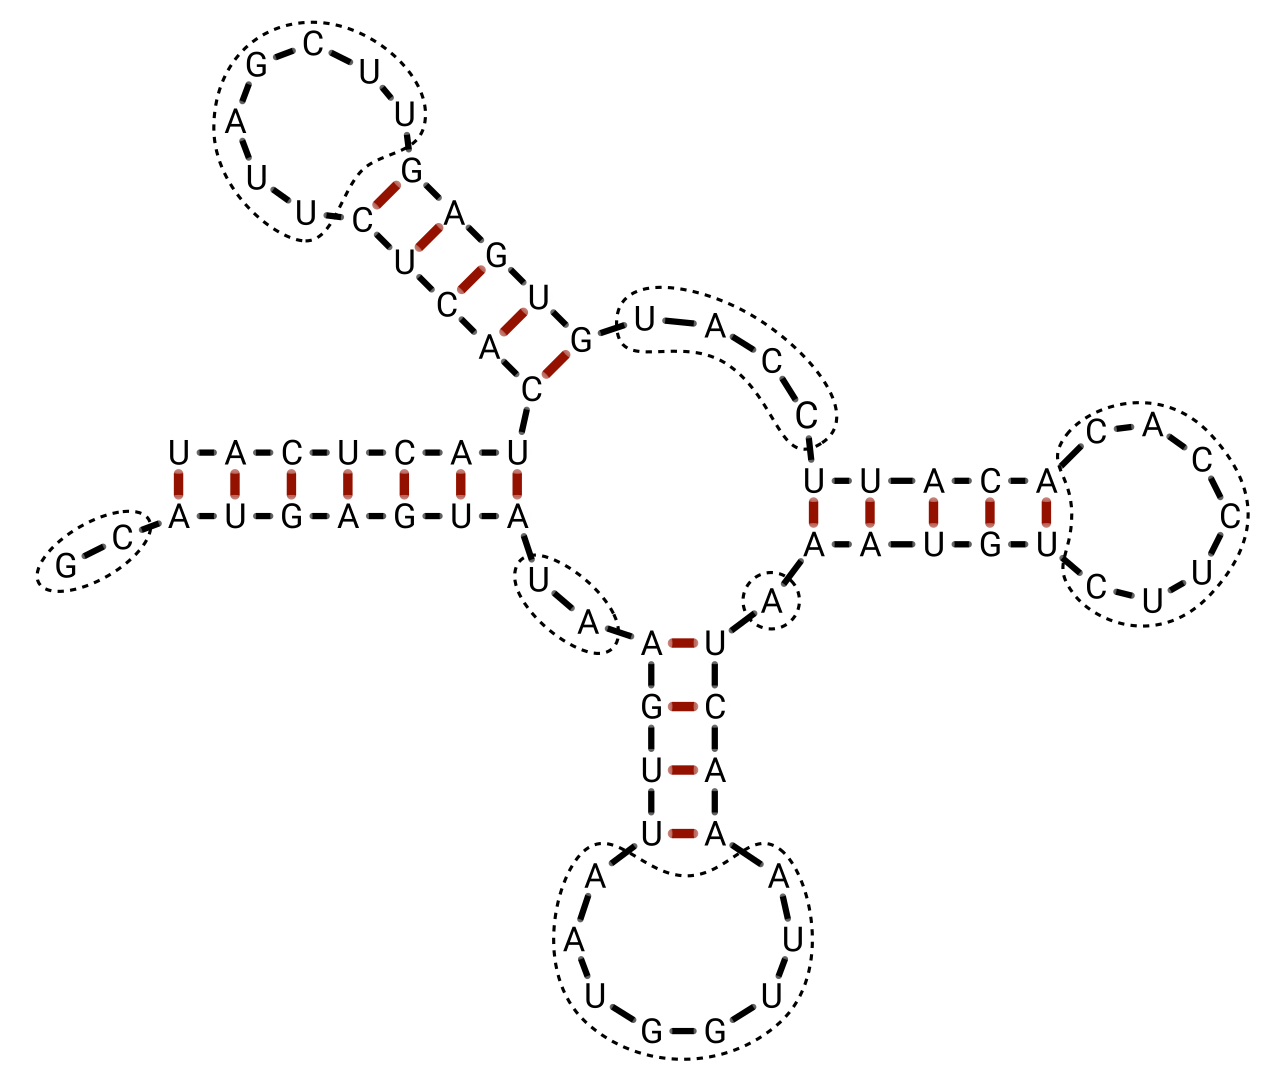
\includegraphics[width=.5\textwidth]{RNA-secondary-structure.png}
    \end{center}
\caption{Beispiel einer RNA Sekundärstruktur mit 21 gebundenen Basenpaaren, die durch die fetten roten Linien gekennzeichnet sind. Lücken sind durch die gepunkteten Kurven gekennzeichnet. Diese Struktur hat eine Bewertung von $2^2+2^2+8^2+1^2+7^2+4^2+7^2=187$.}
\end{figure}
\begin{enumerate}
    \item Beschreibe und analysiere einen Algorithmus, der die größtmögliche \emph{Anzahl} an gebundenen Basenpaaren in der Sekundärstruktur einer gegebenen RNA-Sequenz berechnet.
    \item Eine \emph{Lücke} in der Sekundärstruktur ist ein maximaler Teilstring von ungebundenen Basen. Große Lücken sind chemisch instabil, daher sind Sekundärstrukturen mit kleineren Lücken viel wahrscheinlicher.
    Um diese Präferenz einzubeziehen, definieren wir jetzt die \emph{Bewertung} einer Sekundärstruktur als die Summe der \emph{Quadrate} der Längen aller Lücken; siehe die obige Abbildung. (Diese Bewertung ist fiktional; um die tatsächliche RNA-Struktur vorherzusagen braucht man \emph{deutlich} komplizierte Bewertungsmethoden.)

    Beschreibe und analysiere einen Algorithmus, der für eine gegebene RNA-Sequenz die kleinstmögliche Bewertung einer Sekundärstruktur berechnet.
\end{enumerate}

\paragraph{Hinweise zur Abgabe.}
Im Buch [\href{https://jeffe.cs.illinois.edu/teaching/algorithms/book/Algorithms-JeffE.pdf}{Erickson}, Abschnitt 3.4] ist in kleinen Schritten beschrieben, wie man bei dynamischer Programmierung vorgeht.
Folge diesen Schritten!
Fang gar nicht erst an, über for-Schleifen nachzudenken, bevor du eine vollständige rekursive Lösung hast! Das beinhaltet eine klar verständliche deutsche oder englische Spezifikation der rekursiven Teilprobleme, die du löst (ohne diesen Teil erhältst du keinen \emoji{star}).
In der Algorithmenentwicklung, in der Programmierung, und in den meisten Aufgaben des Lebens gilt immer: \textbf{Mach es zuerst korrekt, dann effizient.}
Den \emoji{star} erhälst du für die vollständige und weitgehend korrekte Bearbeitung der beiden Aufgabenteile.

%\input{allgemeine-kriterien.inc}
\end{document}
